\chapter{Testprozess}
\label{testentwurf}

Nachdem wir zuvor festgestellt haben, dass die PrimePfad Abdeckung potenziell das sinnvollste Abdeckungskriterium ist, wollen wir im folgenden
eine Methodik entiwckeln die es erlaubt, mithilfe dieses Abdeckunskriteriums Tests für GraphQL zu entwerfen.
Die zu entwickelnde Methodik wird in einigen Teilen stark an der Methode aus~\cite{property-based-testing} orientiert sein, dies wird
jedoch an den betreffenden Stellen kenntlich gemacht.
In diesem Kapitel wird die Methodik konzeptionell entwickelt und im folgenden Kapitel~\ref{testautomatisierung} ein Prototyp entwickelt, der
die Methodik umsetzt und validiert.
Die zu entwickelnde Methode arbeitet grob nach dem in Abbildung~\ref{methodeablauf} gezeigtem Muster.

\begin{figure}[H]
    \centering
    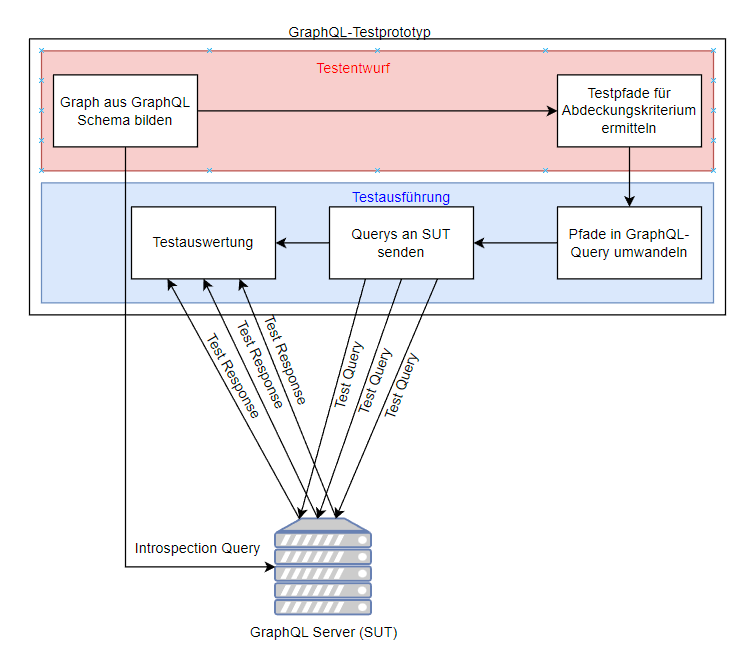
\includegraphics[width=0.75\textwidth,keepaspectratio]{img/fktweiseprototyp}
    \caption{Grober Ablauf des Testprozesses}
    \label{methodeablauf}
\end{figure}

Wie in Abbildung~\ref{methodeablauf} zu sehen ist der gesamte Testprozess in zwei Teile aufgeteilt.
Einerseits in den Testentwurf und andererseits in die Testausführung.
Der Testentwurf basiert auf den zuvor erarbeiteten Theorien und die Testausführung orientiert sich stark am
Property-based Testing \cite[vgl. Method]{property-based-testing}.

\section{Testentwurf}

Der erste Abschnitt des Testprozesses erarbeitet die Pfadgenerierung nach gewähltem Abdeckungskriterium.
Wie zuvor ermittelt, wird die PrimePfad Abdeckung im folgenden ermittelt.
Die Methode erlaubt allerdings auch einen Wechsel des Abdeckungskriteriums da im Endeffekt nur die Pfade für die weiteren Prozesse
genutzt werden können.
Bevor jedoch ein Abdeckungskriterium genutzt werden kann, muss das GraphQL-Schema in einen Graphen übersetzt werden.

\subsection{GraphQL-Schema in Graph abbilden}
\label{schemagraph}

Laut GraphQL-Specification~\cite{graphqlspecification} erlaubt ein GraphQL Server, dass Abfragen über die Schemastruktur des
Servers erlaubt sind \cite[vgl. 4. Introspection]{graphqlspecification}.
Mithilfe einer Introspection-Query \ref{introspection-query} lässt sich das gesamte Schema eines GraphQL-Servers abrufen.
Die Introspection-Query existiert in verschiedenen Varianten, wir nutzen hier die exakt gleiche Version wie sie auch von \cite[]{property-based-testing} genutzt wird.
Ergebnis der Introspection Query ist ein JSON-Objekt mit einer Struktur wie in Listing~\ref{introspec} gezeigt.

\begin{lstlisting}[language=json, caption={Schema-Response},captionpos=b]
    {
        "data": {
            "__schema": {
                "queryType": {},
                "mutationType": {},
                "subscriptionType": {},
                "types": [],
                "directives": []
            }
        }
    }
\end{lstlisting}
\label{introspec}

Der Eintrag $queryType$ gibt den Namen des Typens an, der Startpunkt jeder Query ist, so wie in Kapitel\ref{gqlcov} festgelegt.
Mit dem Eintrag $types$ erhalten wir eine Liste aller Typen wobei jeder Eintrag der Struktur in Listing\ref{typstrukt} entspricht.

\begin{lstlisting}[language=json, caption={Type-Field},captionpos=b]
        {
          "kind": "",
          "name": "",
          "description": "",
          "fields": [],
          "inputFields": [],
          "interfaces": [],
          "enumValues": [],
          "possibleTypes": []
        }
\end{lstlisting}
\label{typstrukt}


Um nun aus dem Schema einen Graphen zu erstellen, benötigen wir die Felder $kind$, $name$, $fields$.
$kind$ ist die Angabe, von welchem Typ das Feld ist.
Hierbei gibt es 9 Möglichkeiten, die dieses Feld annehmen kann.

\begin{itemize}
    \item \textbf{ObjectTypeDefinition (OBJECT):} Repräsentiert ein Objekt mit Feldern.
    \item \textbf{ScalarTypeDefinition (SCALAR):} Eingebaute oder benutzerdefinierte Typen wie \texttt{Int}, \texttt{Float}, \texttt{String}, \texttt{Boolean} und \texttt{ID}.
    \item \textbf{InputObjectTypeDefinition (INPUT\_OBJECT):} Erlaubt das Übergeben komplexer Objekte als Argumente.
    \item \textbf{InterfaceTypeDefinition (INTERFACE):} Repräsentiert eine Liste von Feldern, die andere Objekttypen enthalten müssen.
    \item \textbf{UnionTypeDefinition (UNION):} Kann einen von mehreren Arten von Objekttypen repräsentieren.
    \item \textbf{EnumTypeDefinition (ENUM):} Ein Skalartyp, der auf eine bestimmte Liste von Werten beschränkt ist.
    \item \textbf{ListTypeDefinition (LIST):} Repräsentiert eine Liste von Werten eines bestimmten Typs.
    \item \textbf{NonNullTypeDefinition (NON\_NULL):} Ein Modifikator, der angibt, dass der angewandte Typ nicht null sein kann.
    \item \textbf{DirectiveDefinition (DIRECTIVE):} Passt das Verhalten von Feldern oder Typen  Schema an.
\end{itemize}

Um einen Graphen aus dem Schema zu entwickeln benötigen wir nur Felder vom Typ $OBJECT$.
Die Menge aller Objekte vom Typ $OBJECT$ sind die Menge aller Knoten unseres Graphens.
Um nun die Kanten, also die Beziehungen zwischen diesen einzelnen Knoten zu bekommen müssen wir uns die Defintion
eines Typens näher ansehen.
Wie in $Type-Field$ gesehen, definiert ein Type immer ein Feld $fields$.
In diesem Feld $fields$ verbirgt sich die Informationen aller Kanten, die ausgehend von diesem Knoten sind.
Das Feld $fields$ beeinhaltet Objekte folgender Struktur:

\begin{lstlisting}[language=json, caption={Type-Field},captionpos=b]
            {
              "name": "",
              "description": "",
              "args": [],
              "type": {},
              "isDeprecated": "",
              "deprecationReason": ""
            }
\end{lstlisting}

Wobei für die Kantensuche das Feld type besonders wichtig ist.
Dieses ist wie folgt definiert:

\begin{lstlisting}[language=json, caption={Type-Field},captionpos=b]
    {
        "kind": "",
        "name": "",
        "ofType": null
    }
\end{lstlisting}

Wenn nun der Eintrag $kind$ den Wert $OBJECT$ trägt, so ist klar, dass unser hier definiertes $OBJECT$ eine Kante zum
Knoten $name$ besitzt.

\subsection{Testpfade ermitteln}
\label{testpfade}

Da wir nun einen Graphen passend zum Schema ermittelt haben, gilt es, die Testpfade zu ermitteln, welche die PrimePfad-Abdeckung erfüllen.
Hierzu nutzen wir den in~\cite[Finding Prime Test Paths]{software-testing} vorgestellten Algorithmus.
Dabei werden zuerst die einfachen Pfade ermittelt und dann gefiltert.
Dies sind Pfade ähnlich zu Definition~\ref{primepfad} mit der Lockerung, dass diese Pfade auch Teilpfad eines längeren Pfades sein können~\cite[vgl. S. 35]{software-testing}.
Der längste einfache Pfad kann maximal so lang sein wie die Anzahl der Knoten des Graphens~\cite[vgl. S.41 ]{software-testing}.
Nun wird von jedem Knoten aus expandiert und eine Liste über alle Pfade geführt.
Pfade werden nicht weiter expandiert, wenn diese einen Knoten doppelt enthalten.
Endergebnis ist dann eine Liste aller einfachen Pfade.
Filtert man die einfachen Pfade heraus, die Teil eines anderen Pfades sind erhält man nach Definition~\ref{primecov} die PrimePfad Abdeckung da
wir alle PrimePfade gefunden haben denn es gilt, dass die Menge der Primepfade eine echte Teilmenge der einfachen Pfade ist~\cite[vgl. S. 35]{software-testing}.
Mit der Einschränkung von GraphQL, dass valide Querys stets im Query-Knoten starten müssen, muss sichergestellt werden, dass die PrimePfade dort starten.
Um dies umzusetzen legen wir fest, dass der kürzeste Weg vom Query Knoten zum Startknoten des PrimePfades zu ermitteln ist und an den PrimePfad anzuhängen,
sodass aus diesem später eine valide Query generiert werden kann.

\section{Testausführung}

Die ermittelten Pfade werden nun zu validen GraphQL-Querys umgewandelt und dann ausgeführt um den Test zu validieren.
Die Pfadumwandlung in eine valide Query ist noch methodisch stark abweichend zu \cite{property-based-testing}.
Die späteren Schritte, also Test ausführen und auswerten sind methodisch gleich zu \cite{property-based-testing}.

\subsection{Pfade in Query umwandeln}
\label{pfadquery}

Einen Pfad wandeln wir in eine konkrete Query um indem wir die Typinformationen aus dem Schema nutzen.
Beginnend im Query-Knoten wird der Pfad iteriert.
Das GraphQL-Schema enthält Informationen darüber, welche Informationen nötig sind um zum nächsten adjazenten Knoten des Pfades zu kommen.
Die Informationen darüber sind im Eintrag $fields$ enthalten wie in Listing~\ref{typstrukt} gesehen.
Im $fields$ Eintrag steht dann, ob eine Kante Argumente benötigt und welcher Typ das Rückgabeobjekt ist.
Das Rückgabeobjekt des $fields$ steht dabei aber schon fest da dieser exakt gleich sein muss mit dem nächsten Knoten des Pfades.
In jedem Schritt der Query-Generierung werden stets alle Felder vom Typ $SCALAR$ hinzugefügt, damit sichergestellt werden kann, dass
der Typ alle Felder implementiert hat.
Je nach Implementierung können durch die Feldauswahl weitere Funktionen abgefragt werden, daher inkludieren wir schlichtweg alles.
Felder vom Typ $OBJECT$ werden nur zur Query hinzugefügt, wenn der Typ des $OBJECT$ dem nächsten Knoten entspricht.
Im Allgemeinen lässt sich das Verfahren in diesem Pseudocode darstellen: \\

\begin{verbatim}
    path = (A , B , ..... , Y)
    query = {}

    while path not empty:
        knoten = pfad.pop()
        ScalarFields = getScalarFields(knoten)
        query.addScalars(ScalarFields)
        edge = pfad.peek()
        args = checkForEdgeArgs(edge)
        query.addArgs(args)
    return query
\end{verbatim}

Die Argumente die in einer Query verwendet werden, sind stets nur $SCALAR$ Types und somit einfache Datentypen.
Es gibt verschiedene Arten die Argumentgeneratoren umzusetzen, vorerst werden diese jedoch methodisch exakt wie in \cite{property-based-testing} genutzt.
Dabei wird der Typ des Arguments genutzt um zufällig ein Argument des entsprechenden Typens zu generieren.
Ergebnis des Prozesses ist schließlich eine valide GraphQL-Query.
In einer konkreten Implementierung ist die Syntax von GraphQL zu beachten, diese ist einsehbar in \cite[2.3 Language Operations]{graphqlspecification}.

\subsection{Querys an SUT senden}
\label{testf}

Die generierten Querys stellen die konkreten Tests für GraphQL dar.
Um diese auszuführen, werden alle generierten Querys per \textit{HTTP-POST} an den GraphQL-Server geschickt und die Antworten
werden gespeichert, dies ist analog zu \cite{property-based-testing}.
Es ist wünschenswert, dass die generierten Querys in einem Testframework abgebildet und gespeichert werden.
Dadurch werden die Tests reproduzierbar und können später verwendet werden um etwaige Fehlerbehebungen zu verifizieren.

\subsection{Testauswertung}

Die Auswertung der Tests basiert im Grunde auf den selben Annahmen wie Sie in \cite{property-based-testing} getroffen wurden.
Dabei werden die HTTP-Codes der Antworten und die existierenden Keys in der Response überprüft.
Eine Antwort eines GraphQL-Server liefert stets einen Statuscode \textbf{200} wenn kein kritischer Fehler auftrat.
Kritische Fehler sind stets ein Statuscode \textbf{500} \cite[vgl. 7. Response]{graphqlspecification}.
Daher wird jede Antwort mit einem Code \textbf{500} als gefundenere Fehler und fehlerhafter Test betrachtet.
Eine Antwort mit einem Statuscode \textbf{200} kann jedoch auch Fehler aufweisen.
Dies wird ersichtlich durch einen zweiten Haupteintrag $errors$ in einer Antwort, ersichtlich in Listing~\ref{err}

\begin{lstlisting}[language=GraphQL, label={err}, caption={fehlerhafte Antwort}]
    {
        "data": {}
        "errors": {}
    }
\end{lstlisting}

Hierbei müssen die $errors$ jedoch manuell geprüft werden ob es sich um wirkliche Programmierfehler handelt oder gewünschtem Verhalten,
da die Zufallsargumente teilweise dafür sorgen, dass Konventionen nicht eingehalten werden können.
Die Zufallsargumente sorgen allerdings auch dafür, dass die errechnete PrimePfad Abdeckung nicht praktisch umgesetzt wird.
Sehr häufig kommt es vor, dass zufällig generierte Argumente schon in den Anfängen des Pfades nicht passend zu den unterliegenden Daten sind.
Dadurch folgt, dass ein Großteil der Testpfade die theoretisch eine gute Abdeckung aufweisen, praktisch diese Abdeckung nicht erreichen.
Um Messen zu können, ob ein Pfad seine theoretische Abdeckung auch praktisch erreicht, führen wir eine Abschätzung darüber ein.

\subsubsection{Abschätzung der Pfadlängen}
Diese Methode verbessert zwar nicht die Testergebnisse allerdings gibt Sie uns Informationen darüber wie viel von unserem Pfad in Wirklichkeit
abgedeckt wurden.
Dadurch lässt sich der Erfolg der Tests besser abschätzen da wir so messen können, ob die Querys wirklich die Funktionen ausgeführt haben.
Hierzu wird die Pfadlänge des Pfades der zur Erstellung der Query genutzt wurde als erwartete Pfadlänge angenommen.
Die Pfadlänge der Antwort wird dann als tatsächliche Pfadlänge genommen.
Der Unterschied zwischen erwarteter und tatsächlicher Pfadlänge ist dann unser Auswertungsmerkmal für diesen speziellen Test.
Die Pfadlänge der Response ist die maximale Tiefe der JSON-Response verringert um 1.

\[ \text{Tiefe des Pfades} = \text{Tiefe des JSON-Response-Objekts} - 1 \]

Demnach hätte folgende Response eine Tiefe von 2
\begin{lstlisting}[language=GraphQL, caption={vollständige Response}]
    {
        "data": {
            "book": {
                id: "1",
                title: "Moby Dick"
                publisher: {
                    id: "1",
                    name: "Testverlag"
                }
            }
        }
    }
\end{lstlisting}

Und die leere Antwort hätte eine Tiefe von 1

\begin{lstlisting}[language=GraphQL, caption={mangelhafte Response}]
    {
        "data": {
            "book": null
        }
    }
\end{lstlisting}

Obwohl eine leere Response zulässig ist und nicht auf einen Fehler hindeutet, signalisiert uns der Unterschied zwischen erwarteter und tatsächlicher Länge dann,
ob die Query tatsächlich alle Resolver ausgeführt hat oder nur einen Teil davon.
Hierdurch können wir die Tests in ihrer Qualität auswerten.
Wir können die Pfadlängen aller erwarteten Pfade addieren, das gleiche müssen wir auch mit den tatsächlichen Pfadlängen machen.
So erreichen wir zwei Zahlen und mit diesen können wir eine prozentuale Einschätzung abgeben, wieviel Prozent unserer Tests
insgesamt ausgeführt wurden.
Wir rechnen hierfür:

\[ \text{Prozent der tatsächlichen Abdeckung} = \frac{\text{tatsächliche Gesamtpfadlänge}}{\text{erwartete Gesamtpfadlänge}} * 100 \]

Wir sollten einen Wert von 100\% anstreben.
Dies würde bedeuten, dass unsere generierten Tests auch alle Funktionen getestet haben.
Andernfalls bedeutet ein Prozentsatz unter 100\% eben, dass nicht alle Funktionen tatsächlich von den Querys überdeckt wurden.

\\
\\

Abschließend wollen wir noch kurz erläutern, wie es möglich wäre, die Tatsächliche Abdeckung zu erhöhen.
Dies geschieht vor allem durch ein anpassen der Zufallsgeneratoren und die Anzahl der Querys.

\subsubsection{Zufallsgeneratoren der Argumente}
\label{zufallsgen}

Die zuvor vorgestellte Abschätzung liefert uns einen Hinweis darauf, wie gut unsere Querys tatsächlich getestet haben.
Ein Ansatz der die Querys eine bessere tatsächliche Abdeckung zu erreichen lässt ist das anpassen der Generatoren für die Argumente.
In der vorgestellten Methode in Kapitel~\ref{pfadquery} erstellen wir komplett zufällig Argumente für die Funktionen.
Dies bedeutet, dass z.B. der Type $ID$ als String gewertet wird.
Dieser Type ist in der Realität jedoch eingeschränkt und gleichzeitig sehr bedeutend, da dieser häufig als Argument angegeben wird und er eine spezielle Struktur hat.
Es hängt natürlich stark von der eigenen Implementierung der GraphQL-API ab allerdings wenn in der Implementierung
eine $ID$ definiert ist als Zahlenstring, so kann es sich durchaus lohnen, dass der Argumentgenerator für die ID auch speziell
auf Zahlenstrings angepasst wird.
Alternativ kann auch eine Liste aller existenten IDs angegeben werden und zufällig ausgewählt werden.
Die Anpassung der Argumentgeneratoren an die zugrundeliegenden Daten ist höchst spezifisch und daher kann keine allgemeine
Vorgehensweise ermittelt werden.
Ziel der Anpassung ist es, dass die Chance erhöht wird mit der Argumente zufällig generiert werden, die dann tatsächlich zu Zugrunde liegenden Daten passen.

\subsubsection{Anzahl der Querys}

Die Wahrscheinlichkeit passende Argumente zu generieren steigt außerdem mit der Anzahl an generierten Querys.
Erhöht man die Anzahl an generierten Querys pro PFad, so erhöht sich auch die Wahrscheinlichkeit, dass zumindest ein Pfad
eine gute Abdeckung erreicht.
Hierfür müssen wir die Methode aus Kapitel~\ref{pfadquery} so oft wie gewünscht wiederholen, sodass wir verschiedene Querys mit verschiedenen Argumenten erhalten.
Bei dieser Methode ist wichtig, dass sich die Argumente der Querys verändern da wir sonst einfach mehrfach die selbe Query stellen mit der
gleichen zu erwartenden Antwort.
Zusammen mit den angepassten Argumentgeneratoren kann so das zufallsbasierte Argumentgenerieren ein wenig begrenzt werden
und es ist wahrscheinlicher, dass gute Tests entstehen.

\section{Zusammenfassung der Methode}

Wir wollen im folgenden die eben vorgestellte Methode noch einmal kurz zusammenfassen damit diese übersichtlicher wird.
Unsere hier vorgestellte Methode funktioniert so wie in Abbildung~\ref{methodeablauf} gezeigt.
Wie zu sehen, ist der ganz grobe Ablauf ähnlich zum~\cite[Property-based Testing]{property-based-testing} allerdings unterscheidet sich die
Methode in einigen Teilen sehr stark vom~\cite[Property-based Testing]{property-based-testing}.
Wir fügen in unserer Methode den Schritt hinzu, dass wir einen Graphen erstellen welcher die Knoten und Kanten des GraphQL-Schemas repräsentiert
während in~\cite[Property-based Testing]{property-based-testing} ausgehend vom Query-Type zufällig bis zu einer bestimmten Pfadlänge (dem Rekursionslimit)
die Pfade gebildet werden, indem immer zufällig Felder hinzugefügt werden.
Durch unsere Methode erreichen wir, dass Pfade jeder Länge, die durchaus länger sein können als ein definiertes Rekursionslimit, abgedeckt werden und
somit die Tests eine bessere Abdeckung erreichen können.
Unser Ansatz erlaubt es außerdem, verschiedene Abdeckungskriterien zu implementieren.
So ist man nicht gezwungen auf einer Methode zu verharren, sondern kann je nach Implementierung die Pfadgenerierung anpassen nach den individuellen
Anforderungen ohne, dass in anderen Schritten etwas geändert werden muss.
Bei der Umwandlung der Pfade in Querys unterscheidet sich unser Ansatz ein wenig von \cite[Property-based Testing]{property-based-testing}.
In unserer Methode generieren wir aus dem Pfad direkt die Query und generieren die nötigen Argumente ''on-the-fly'' während sie erkannt werden.
Im Property-based Ansatz wird ein Datenobjekt als ganzes erstellt, dass die Query später generieren kann.
In der technischen Umsetzung unterscheiden sich beide Methoden, im Ergebnis bekommen Sie jedoch strukturell gleiche Querys.
Die Ausführung der Tests hingegen unterscheidet sich überhaupt nicht mehr zum \cite[Property-based Testing]{property-based-testing}.
Die Einführung der erwarteten gegenüber der tatsächlichen Pfadlänge ist ein neuer Ansatz, der die Qualität der zu testenden Querys
messbar macht - dies fehlt im~\cite[Property-based Testing]{property-based-testing}.
Dort ist man im unklaren darüber wie gut die Tests genau getestet haben und ob die erwartete Abdeckung auch mit der tatsächlichen Übereinstimmt.
\\
\\
Wir haben nun unsere Methode im groben vorgestellt und Unterschiede zum schon bestehenden Ansatz~\cite[Property-based Testing]{property-based-testing} erörtert.
Im folgenden wollen wir uns der praktischen Umsetzung dieser Methode widmen und einen Prototypen entwickeln.
Dieser Prototyp soll dann gegen das~\cite[Property-based Testing Tool]{property-based-testing} antreten und möglichst zeigen, dass die eben entwickelte Methode
eine Verbesserung darstellt.






